\documentclass{slide}
% \usepackage{pgfpages}

% \setbeameroption{show notes on second screen}

\title{Microkernel Architecture}
\subtitle{CSSE6400}
\author{Richard Thomas}
\date{\week{3}}

\usepackage{languages}
\usepackage{marvosym}
\usepackage{tikz}
\usetikzlibrary{positioning}
\usetikzlibrary{arrows}
\usetikzlibrary{fit}

\begin{document}

\maketitle

\point[So far\dots]{%
\begin{description}
    \item[Simplicity] -- Monolith, Pipeline
    \item[Modularlity] -- Layered, Pipeline
\end{description}}
\note{Emphasise quality attributes and how architectural styles deliver those attributes.}

\definition{Extensibility}{Features or extensions can be easily added to the software over its lifespan.}

\questionanswer{How easy is it to extend \highlight{Monolith}, \highlight{Layered} or \highlight{Pipeline}?}
{\begin{description}
    \item<2->[Monolith] -- Everything in one container ~\Frowny{}
    \item<3->[Layered] -- Typically all layers ~\Frowny{}
    \item<4->[Pipeline] -- Create a new filter ~\Smiley{}
\end{description}}
\note{Discuss issues of extending a monolith or layered architecture.}

\definition{Interoperability}{Software can easily share information and exchange data with internal components and other systems.}

\questionanswer{What about interoperability?}
{\begin{description}
    \item<2->[Monolith] -- Everything in one container
    {\Large\begin{itemize}
        \item Internal ~\Smiley{}
        \item External ~\Frowny{}
    \end{itemize}}
    \item<3->[Layered] -- Nearest Neighbour
    {\Large\begin{itemize}
        \item Internal ~\Smiley{}
        \item External ~\Frowny{}
    \end{itemize}}
    \item<4->[Pipeline] -- Standard Interface
    {\Large\begin{itemize}
        \item Internal ~\Smiley{}
        \item External ~\Frowny{}
    \end{itemize}}
\end{description}}
\note{Discuss issues of broad interoperability.}

\questionanswer{What if I want simplicity, extensibility and interoperability?}
{Microkernel Architecture}

\definition{Microkernel Architecture}{Core system providing interfaces that allow plug-ins to extend its functionality.}

\begin{frame}{Microkernel Architecture}
\centering
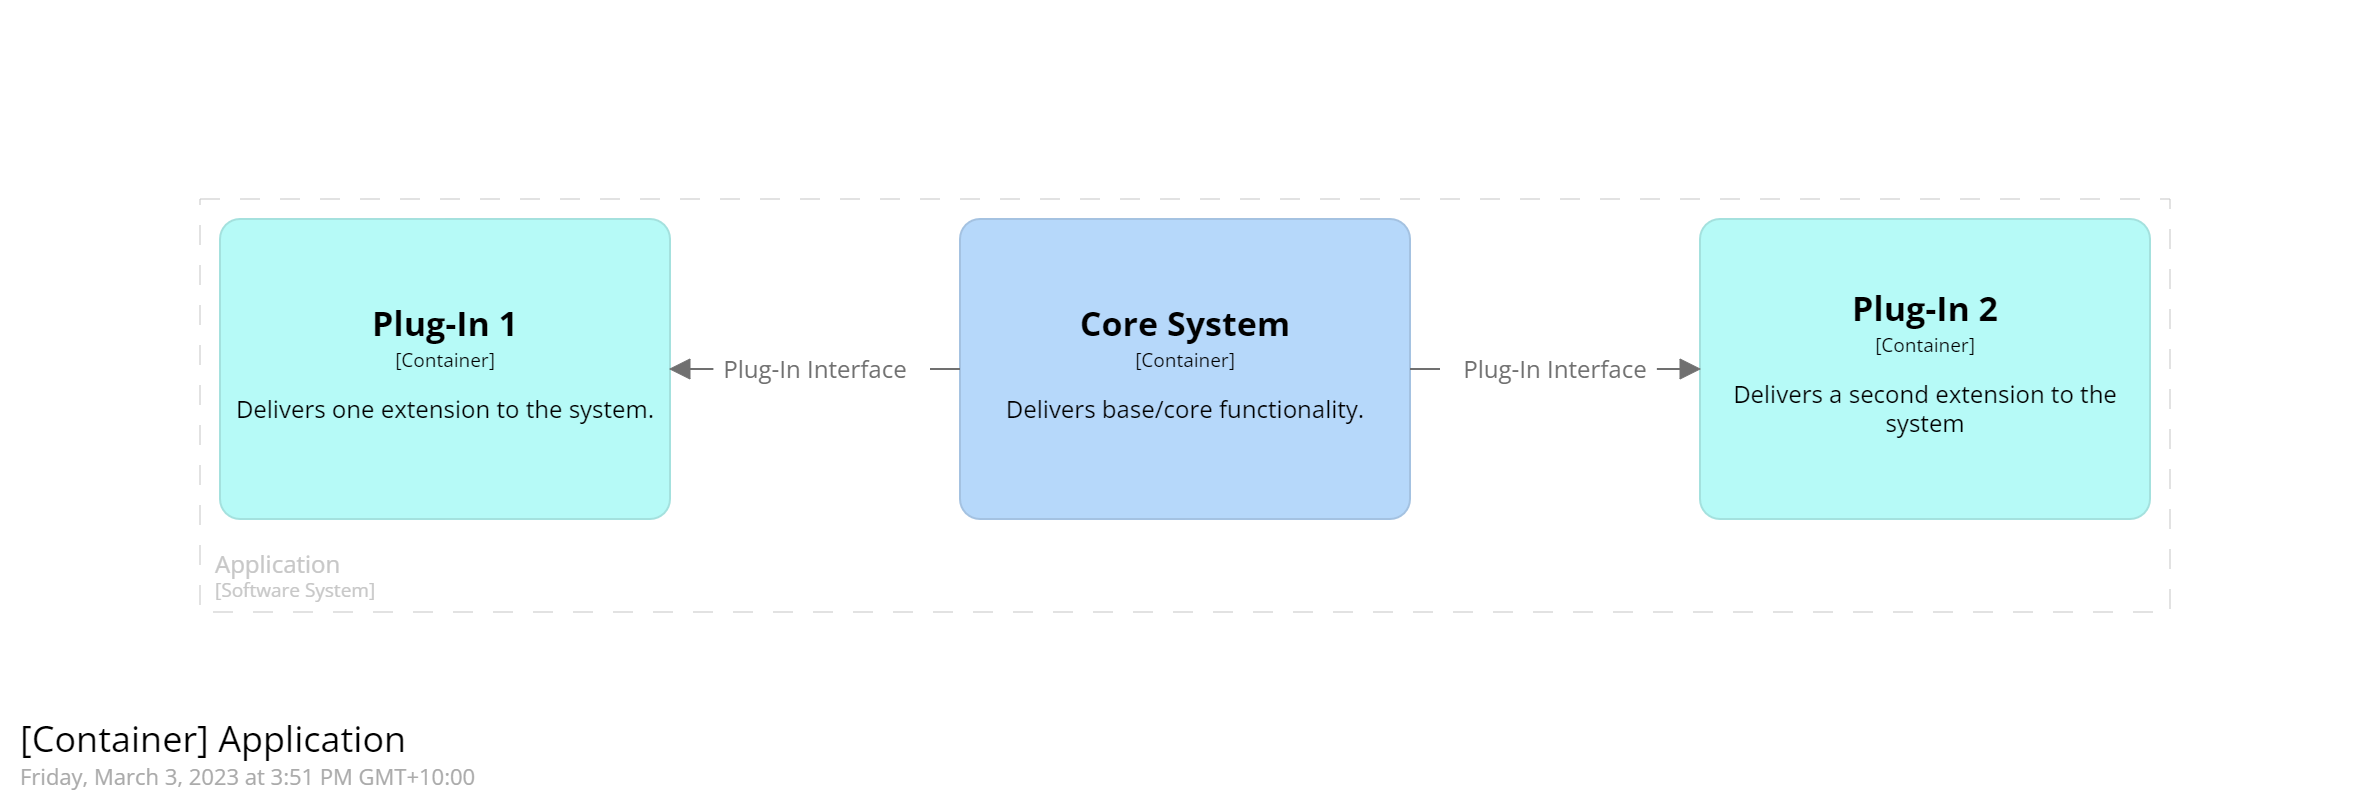
\includegraphics[trim=38 180 22 50,clip,width=\textwidth]{../../notes/microkernel/diagrams/generic-microkernel.png}
\end{frame}

\questionanswer{Can you think of a \highlight{microkernel archiecture}?}{How about \highlight{IntelliJ}?}

\note[itemize]{
    \item Eclipse
    \item ??
}

\references{articles,books}

\end{document}